\documentclass{article}
\usepackage[spanish]{babel}
\usepackage{graphicx}
\usepackage{xcolor}
\usepackage[utf8]{inputenc}
\usepackage{fancyhdr}
\usepackage{lastpage}
\usepackage{enumitem}
\usepackage{listings}
\usepackage{verbatim}
\usepackage{float}

\pagestyle{fancy}
\fancyhf{}
\rfoot{Page \thepage\hspace{1pt} de~\pageref{LastPage}}

\title{Tarea 4}
\author{Guillermo López García}
\begin{document}
\maketitle

\textbf{1º Ejercicio.}
He aquí la solución:

\begin{figure}[H]
\centering
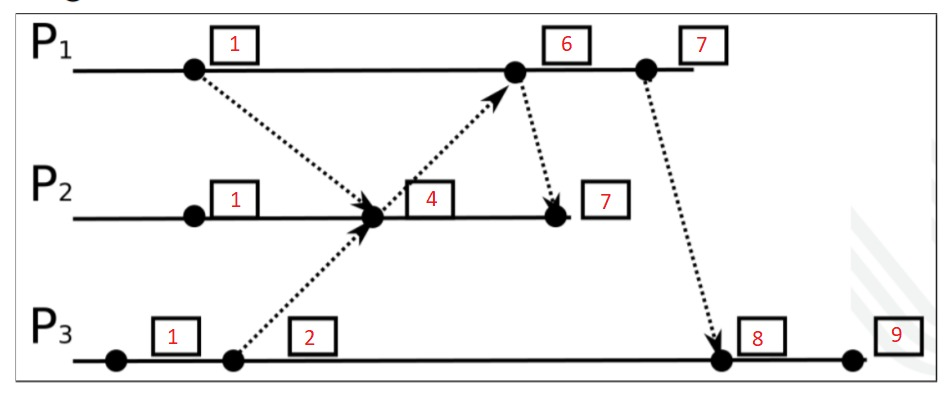
\includegraphics[width=0.7\linewidth]{./lamport}
\caption{Solución al problema con el algoritmo de lamport}
\end{figure}

\textbf{2º Ejercicio.}
Código relevante:
\lstset{
  language=Python,
  texcl=true,
  basicstyle=\ttfamily,
  columns=fullflexible,
  frame=single,
  breaklines=true,
  postbreak=\mbox{\textcolor{red}{$\hookrightarrow$}\space},
}
\lstinputlisting[]{server.py}
\lstinputlisting[]{tools.py}
\lstinputlisting[]{client.py}

\end{document}
